\documentclass[a4paper,10pt]{article}
\usepackage[utf8]{inputenc}
\usepackage[english]{babel}
\usepackage{indentfirst}
\usepackage{listings}
\usepackage{graphicx}
\usepackage{blindtext}
\usepackage{enumitem}
\usepackage{hyperref}
\usepackage[top=2.5cm,bottom=2.5cm,left=2.5cm,right=2.5cm]{geometry}
\pagestyle{headings}
\title{Ftp server in a datadiode}
\author{Rusu George, Boulif Ilias, Orinx Cédric}
\date{\today}

\begin{document}
\maketitle
\newpage
\tableofcontents
\newpage
\section{Concept of operations}
\subsection{Introduction to the problem}
Our client would want to prevent his research and development labs against industrial espionage and confidential information leaking. He wants to divide the company network in order to maintain the labs in an isolated environment. Thus, the critical data could not leave the company using the network. One problem related is assuring that all the operating systems are up to date. This could be achieved using a manual operation where an employee would manually update every node in the isolated network using a mass-storage device\footnote{A USB-key for instance.}. However, this is not the most optimized way and for sure it is not cost less and timeless for the company, without mentioning that there could be dependency problems. This method is prone to human errors and this could generate security vulnerabilities.

\subsection{Our solution}
In order to address this problem we are going to implement a data diode. In electronics as shown in Figure \ref{fig:diode}, a diode is a component which conduct the current in one direction. Thus the term of data diode is a set of components that only let the data to travel in an unidirectional way. An example of use case is illustrated in Figure \ref{fig:datadiode}, letting the data pass from a low risk VLAN\footnote{IEEE 802.1Q.} to a high risk VLAN but not the way around.
\begin{figure}
\centering
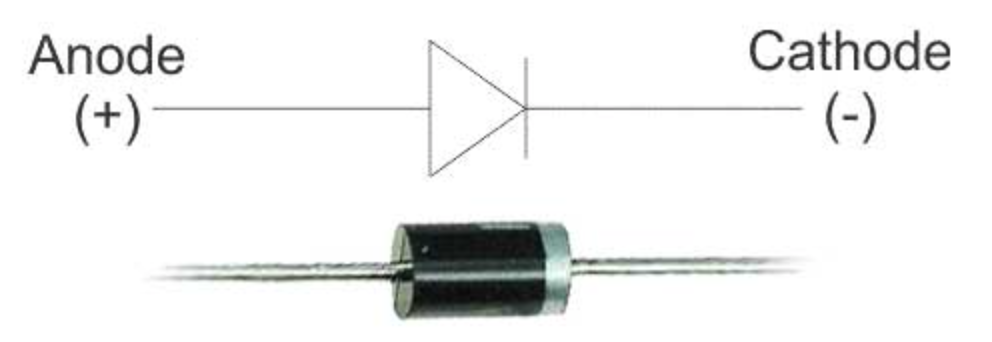
\includegraphics[scale=0.25]{images/diode.png}
\caption{A diode schema in electrionics.}
\label{fig:diode}
\end{figure}

\begin{figure}
\centering
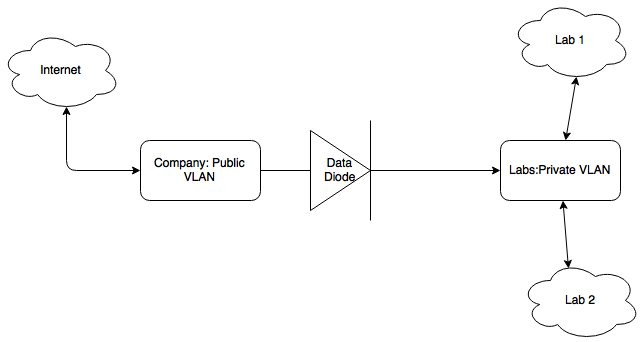
\includegraphics[scale=0.45]{images/dataDiode.png}
\caption{The schema of the usage of a data diode in a company network.}
\label{fig:datadiode}
\end{figure}

A data diode is made using one transmitter(Tx) and one receiver(Rx) both linked using only one fiber cable. Thus, when a digital data is send trough, every bit will be converted\footnote{Using a Digital to analog converter (DAC).} into an electrical pulse which will be convert in light pulse using a LED\footnote{Light Emitting Diode.}. Then, the output light will pass trough the fiber cable and as soon as the photons are reaching the receiver, they will be converted firstly into an electrical pulse by a photo diode and then in bits\footnote{Using an analog to digital converter (ADC).}. Since there is only one fiber, data can only travel in one way.

One major problem of this system is the network transport protocols(layer 4 in the OSI model) that applications are using. The most used transportation protocol nowadays is TCP. However, TCP is a bi-directional protocol which need the 3 way handshake in order to start a connection, thus there must be at least two fiber cables. In contradiction, UDP does not require a handshake process because it does not provide reliability, ordering, data integrity and does not set up a dedicated end-to-end connection automatically. Thus, UDP protocol does not necessary require a bi-directional data transfer. Therefore, the use of such a protocol is recommended when dealing with applications that are not sensitive to data loss or that implements an error checking system. Hence, the UDP protocol is used within the data diode.

It seems obvious now that the transport protocol used between the transmitter and the receiver of the data diode is UDP. However, this brings multiple problems. One of the problems is how to be able to use applications that requires TCP. Another problem could be the reliability of the digital data transfer in the data diode, how can we ensure that there will not be any data loss during the transfer. We will address to those questions further down in this document.

\subsection{Our System description}
The data diode concept is well orchestrated combination between hardware and software. The data diode is composed of two servers: a transmitter and a receiver. We could consider that the transmitter server is connected to the low security risk VLAN where a connection to the internet is made and where all the employees are connected. The receiver is connected to the high security risk VLAN where all the labs are connected and where critical informations is stored.

The transmission of the information will be from the low side to the high side and blocked the way around as shown in Figure \ref{fig:UDPDD}.

\begin{figure}
\centering
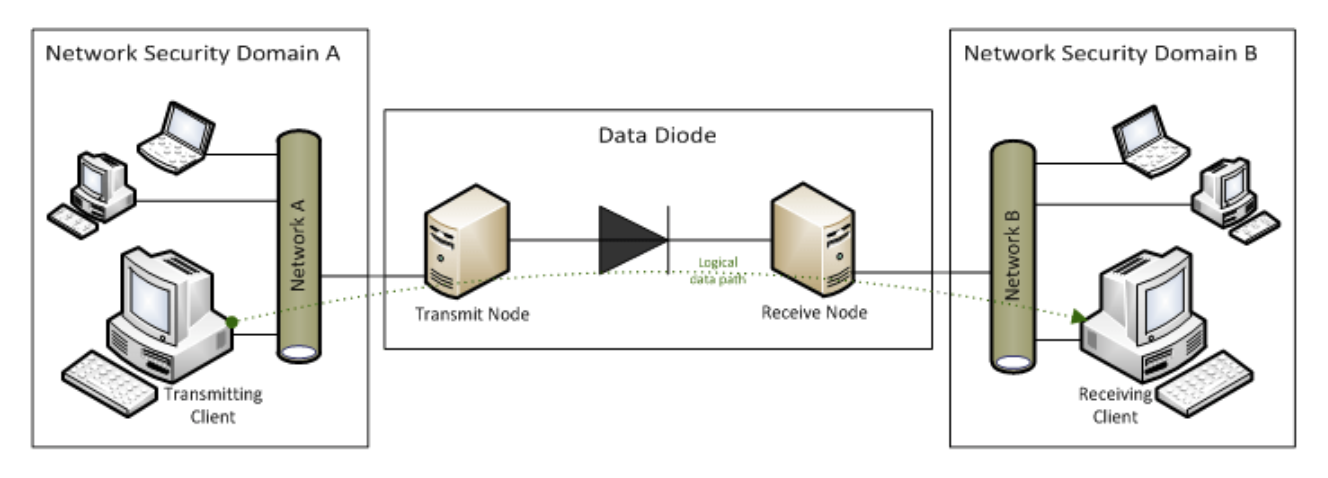
\includegraphics[scale=0.5]{images/logical-scheme-DD.png}
\caption{Data logical path within the data diode.}
\label{fig:UDPDD}
\end{figure}

\subsubsection{Hardware}
The following table presents the components used for the data diode implementation. We should mention that both transmitter and receiver possess two NICs\footnote{Network interface controller.}: one for the communication within the VLAN and one for the data diode.\bigskip
\begin{table}[!h]
\begin{tabular}{|p{3cm}|p{10.5cm}|}
	\hline
	\textbf{Components} & \textbf{Description}                 \\
	\hline
	Transmitter server  &  a physical machine or a virtual machine. The NIC for the data diode will be set in transmission mode only. \\
	\hline
	Receiver server  &  a physical machine or a virtual machine. Similar to the transmission, the nic will only be set in a receiver mode.\\
	\hline
	One fiber/UTP & This optical fiber allows communication between the low server the high server. It will probably be simulated using a UTP/RJ45 cable.\\
	\hline
	4 Fiber NIC/UTP NIC & Two for each server (transmission and receiver).  \\
	\hline
\end{tabular}
\caption{Components description}
\label{tab:component}
\end{table}
\subsubsection{Software}
We have chosen to use Linux as the operating system running on both transmission and receiver servers because of its reputation for safety and performance and also for its stability and efficiency in maintenance.

\paragraph{} A \textbf{web interface} will be used for the administration of the data diode. It will be described in the section \ref{UI}

\paragraph{} \textbf{BlindFTP} is a simple Python script and portable. It will be used for the communication between the two server. It's a tool for transferring files over a unidirectional network link (without acknowledgment), wich is perfect for our data diaode. The absence of acknowledgment is compensated by a redundancy of the data transmitted by UDP. In addition, it is mainly designed to build a network diode type of interconnection. BlindFTP is written in Python language, which allows to obtain a relatively simple code. It has been successfully tested on different operating system, including Linux.

\subsection{Users} 
We will have two types of users in our system : the \textit{administrator} and the \textit{user}.\\

The \textit{administrator} is the person in charge of operating and maintaining the data diode. The only authorized person to interact with the data diode must be one (or two) \textit{administrator} designated by the company. He will have to know how it works and be able to use the administration interface\ref{UI}.\\

The \textit{user} are the employee who are on the secured network and who needs the files
transferred to maintain their computer up-to-date.\\

All users have a type, an username and a password. All these informations are
managed and stored in a database by the company.
\subsection{User Interface}\label{UI}


[idee : site web sur le transmitter, login+ mot de passe , avoir une certainte tracabilité, pouvoir umploader une fichier depuis le site et juste l'envoyer de l'autre cote. ]\\


The administration of our data diode happens through a web interface.
This web interface will be hosted on the transmitter. This will allows to get the
files from the lower network. For the user interface we have tryed to make it
easy to use. In ordre to use the interface, the first step is to log on with his
user name and password.  Once we are connected, (if we are a user??)
we are on a page that allows the file transfer from the transmitter(lower network)
to the receiver(high network), simply by a mechanism of drag and drop(or upload?).
(if we are admin??)

\textbf{TO DO : parler de la tracabilité}


\subsection{System implementation}
\subsection{General usage}
The interface will be used each time by the users from the secured network
in order to transfer a file through the data diode. By using the interface,
users can transfer the files they need by simply dragging and dropping them to
the dedicated transfer folder which is forwarded to the secure network.


\begin{thebibliography}{9}

\bibitem{nist-fips-202}
NIST,
\textit{SHA-3 Standard: Permutation-Based Hash and Extendable-Output Functions},
FEDERAL INFORMATION PROCESSING STANDARDS PUBLICATION,
2015.

\end{thebibliography}
\end{document}